\begin{figure}[htbp]
  \centering
  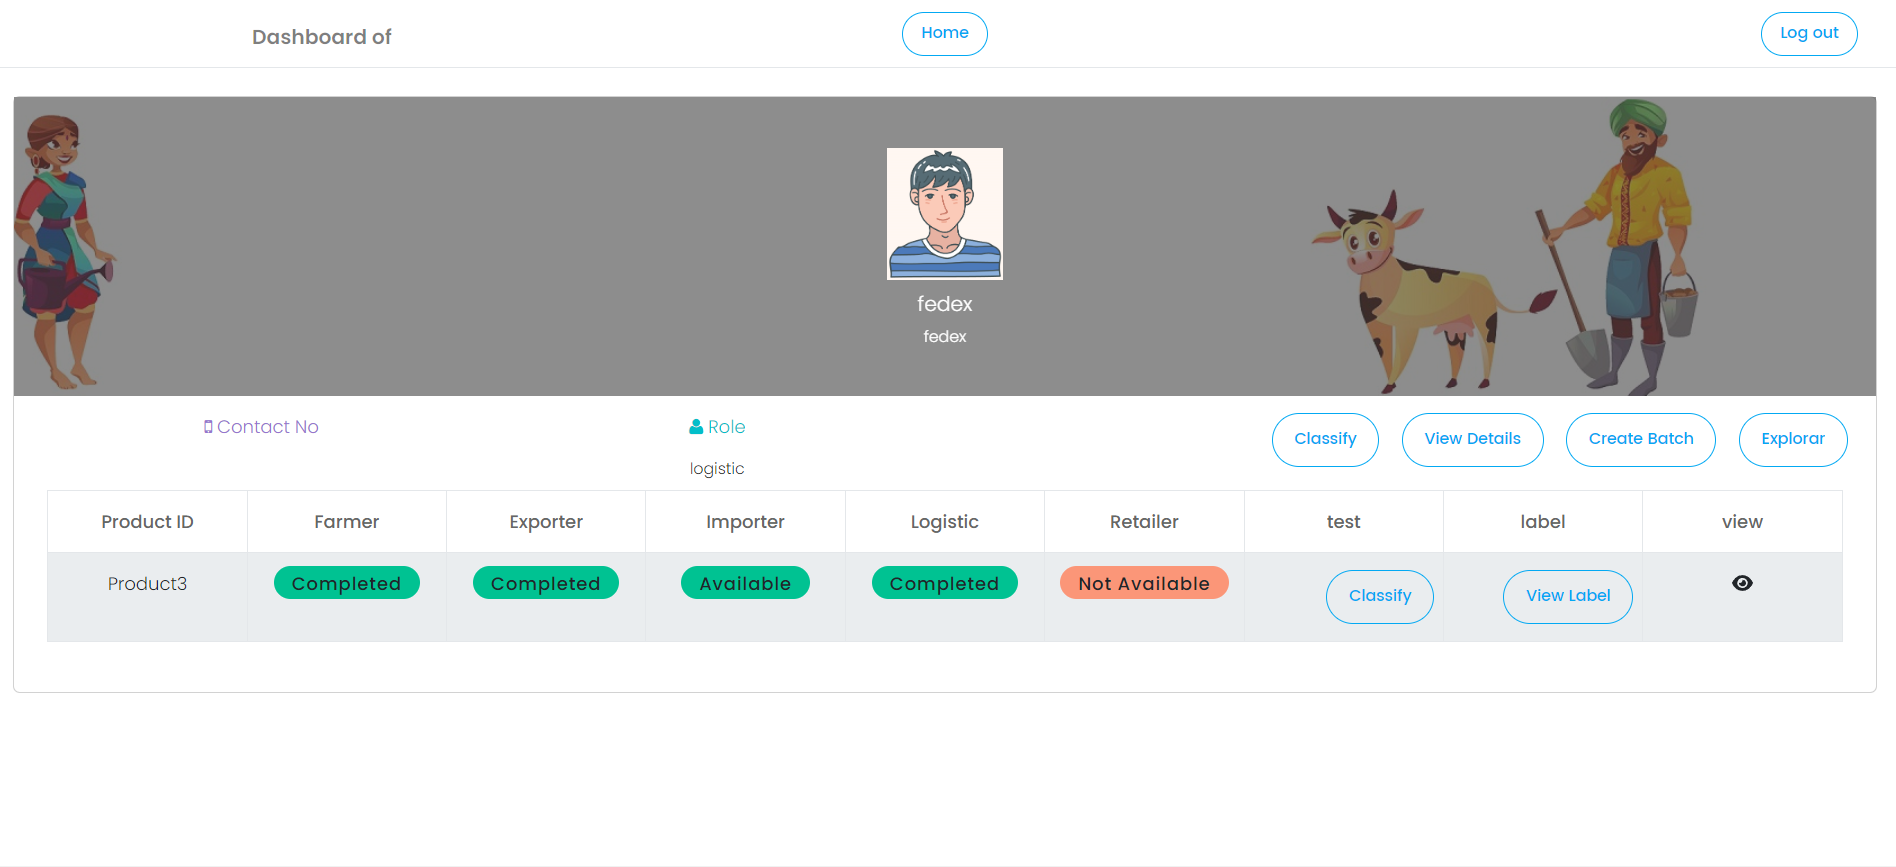
\includegraphics[width=0.9\textwidth]{Chapters/Chapter_7/images/User_interface.png}
  \caption{User Interface }
  \label{fig:figure7_1}
  \end{figure}
\noindent {The Results obtained from  our project is shown with different diagrams provided below\par}
\noindent{The provided user dashboard interface shown in Figure \ref{fig:figure7_1} offers a visually appealing and user-friendly layout for managing products within a supply chain system. Here's a description of the various sections and functionalities:

1. User Information Section:
   - At the top of the dashboard, there is a background image with an overlay.
   - Within the overlay, the user's profile picture, name, and address are displayed.
   - If the user has uploaded a profile picture, it is shown; otherwise, a default image is used.

2. User Details Section:
   - Below the user information, there are sections displaying the user's contact number and role within the system.
   - These details provide quick access to essential user information.

3. Action Buttons:
   - The dashboard includes three action buttons: "Explore," "Create Batch," and "View Details."
   - Clicking the "Explore" button takes the user to a page for exploring products.
   - The "Create Batch" button opens a dialog or form for creating a new batch of products.
   - The "View Details" button allows users to access more detailed information about the system.

4. Product Classification Component:
   - A component related to product classification is present on the dashboard.
   - This component likely provides options or tools for classifying products based on specific criteria.

5. Product Overview Table:
   - The main section of the dashboard features a table presenting an overview of the products.
   - Each row in the table represents a specific product and contains several columns.
   - The columns include the product ID and the parties involved in the supply chain, such as farmers, exporters, importers, logistic providers, and retailers.
   - There are also columns labeled "test," "label," and "view."

6. Dynamic Content and Interactions:
   - The content in the columns of the table dynamically changes based on the product's status and role within the supply chain.
   - Different labels or status indicators, such as "Completed," "Processing," or "Not Available," are displayed to represent the current stage or availability of the product at each role.
   - Users can interact with the table by clicking on specific elements.
   - For example, clicking on the "View" column triggers an action to view more detailed information about the selected product.

In summary, this user dashboard provides an intuitive interface for managing products within a supply chain system. It offers easy access to user information, various functionalities for product management, and a comprehensive overview of products and their statuses.\par }